\hypertarget{__hash__prime_8c}{
\section{\_\-hash\_\-prime.c File Reference}
\label{__hash__prime_8c}\index{_hash_prime.c@{\_\-hash\_\-prime.c}}
}


\subsection{Detailed Description}
\begin{Desc}
\item[For internal use only.]
This file contains the implementation of the \hyperlink{group__dbprim__hash_ga20}{\_\-hash\_\-prime()} function, used to determine a prime number to use as a hash table modulus.\end{Desc}


Definition in file \hyperlink{__hash__prime_8c-source}{\_\-hash\_\-prime.c}.

{\tt \#include \char`\"{}dbprim.h\char`\"{}}\par
{\tt \#include \char`\"{}dbprim\_\-int.h\char`\"{}}\par


Include dependency graph for \_\-hash\_\-prime.c:\begin{figure}[H]
\begin{center}
\leavevmode
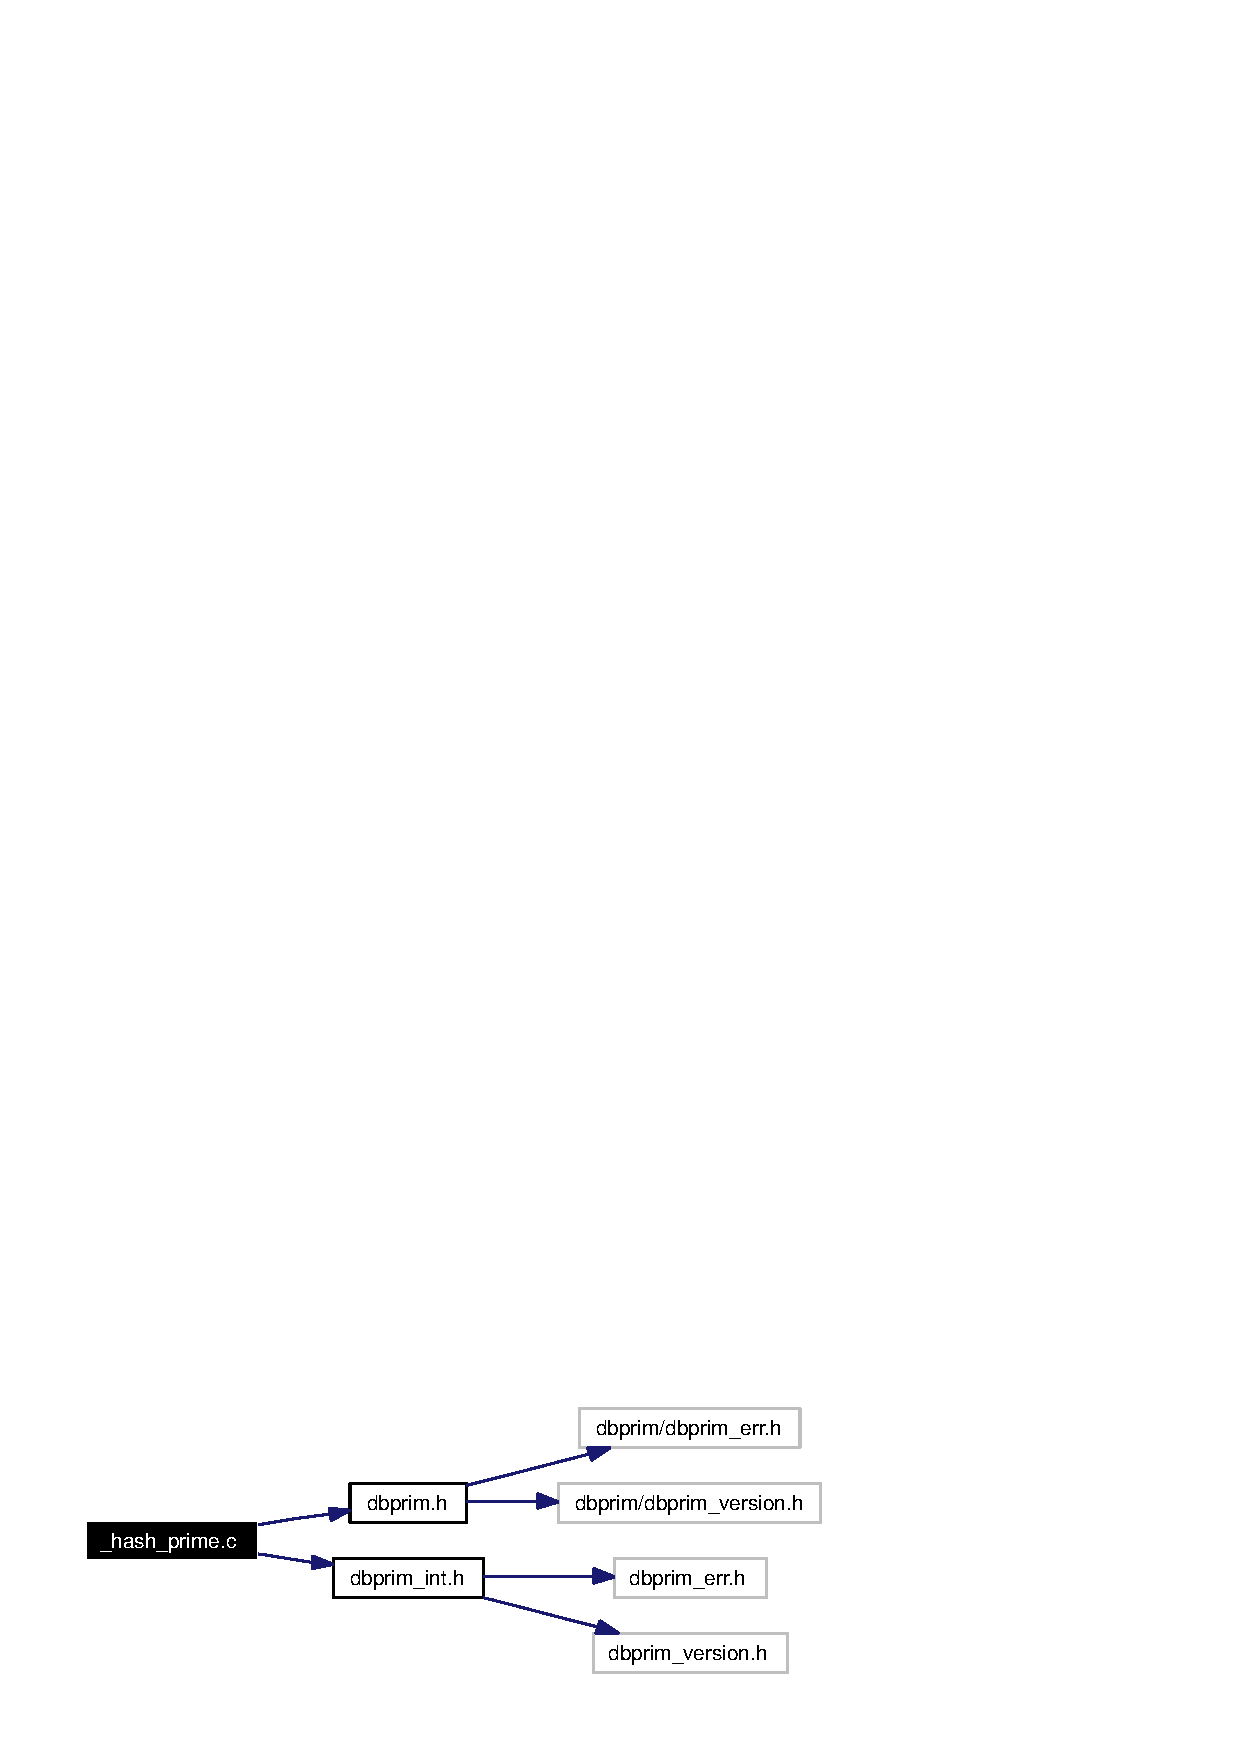
\includegraphics[width=199pt]{__hash__prime_8c__incl}
\end{center}
\end{figure}
\subsection*{Defines}
\begin{CompactItemize}
\item 
\#define \hyperlink{group__dbprim__hash_ga21}{MAX\_\-PRIME}
\begin{CompactList}\small\item\em Largest prime. \item\end{CompactList}\end{CompactItemize}
\subsection*{Functions}
\begin{CompactItemize}
\item 
unsigned long \hyperlink{group__dbprim__hash_ga20}{\_\-hash\_\-prime} (unsigned long start)
\begin{CompactList}\small\item\em Select a prime number. \item\end{CompactList}\end{CompactItemize}
\subsection*{Variables}
\begin{CompactItemize}
\item 
static unsigned long \hyperlink{group__dbprim__hash_ga0}{primes} \mbox{[}$\,$\mbox{]}
\begin{CompactList}\small\item\em Table of primes. \item\end{CompactList}\end{CompactItemize}
